

\begin{frame}
	\frametitle{Planificación}
	
	
	\begin{enumerate}
		\item Septiembre: Estudio del estado del arte y planificación
		\item De octubre a noviembre: desarrollo de la aplicación
		\item De enero a marzo: obtención de resultados
		\item De marzo a mayo: análisis de resultados y redacción
	\end{enumerate}
	\begin{figure}
		\centering
		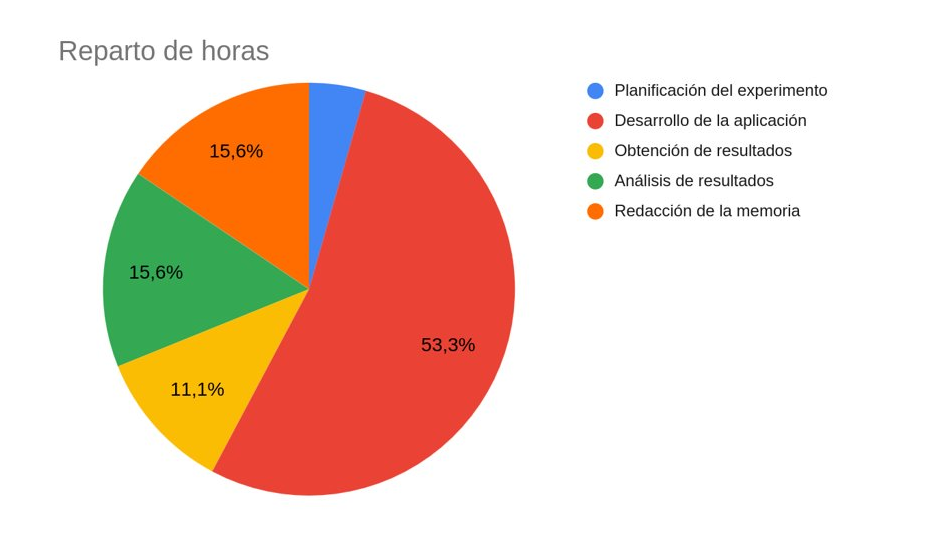
\includegraphics[width=0.8\textwidth]{horas}
	\end{figure}
	
	
\end{frame}

\begin{frame}
	\frametitle{Planificación}
	
	\begin{enumerate}
		\item Contratación personal: 9000\euro
		\item Material: 3000\euro
		\item Desarrollo del experimento: 130\euro
	\end{enumerate}	
	
	\begin{figure}
		\centering
		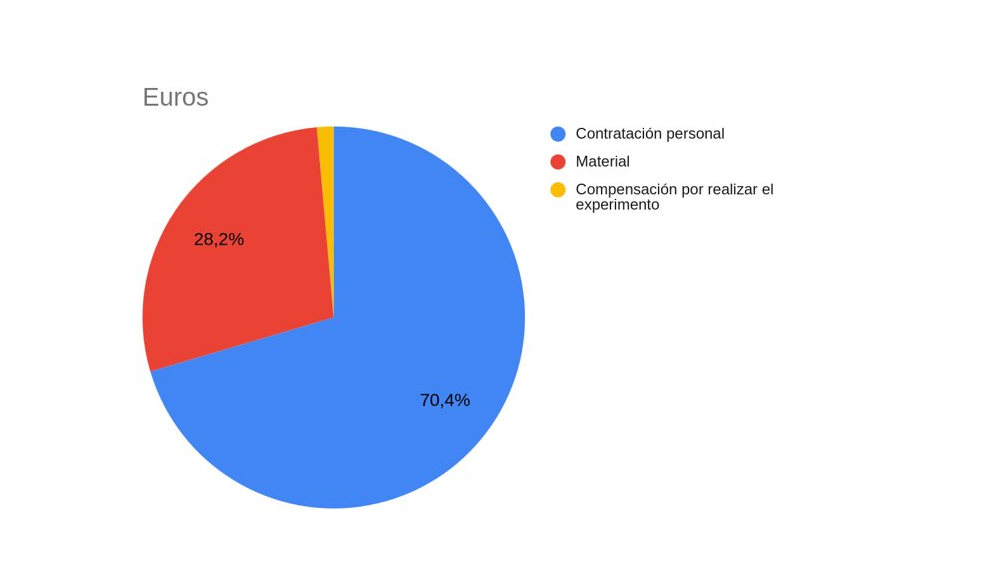
\includegraphics[width=0.8\textwidth]{coste}
	\end{figure}
	
\end{frame}
\begin{frame}
	\frametitle{Parámetros definidos en la Fase de Prueba}
	
	\begin{itemize}
		\item Número de repeticiones por fase. 
		\item Tiempo para la realización del experimento.
		\item Número y disposición de los puntos objetivo.
		\item Puntos en orden o de forma aleatoria.
	\end{itemize}	
	\begin{figure}
		\centering
		\subfloat{
			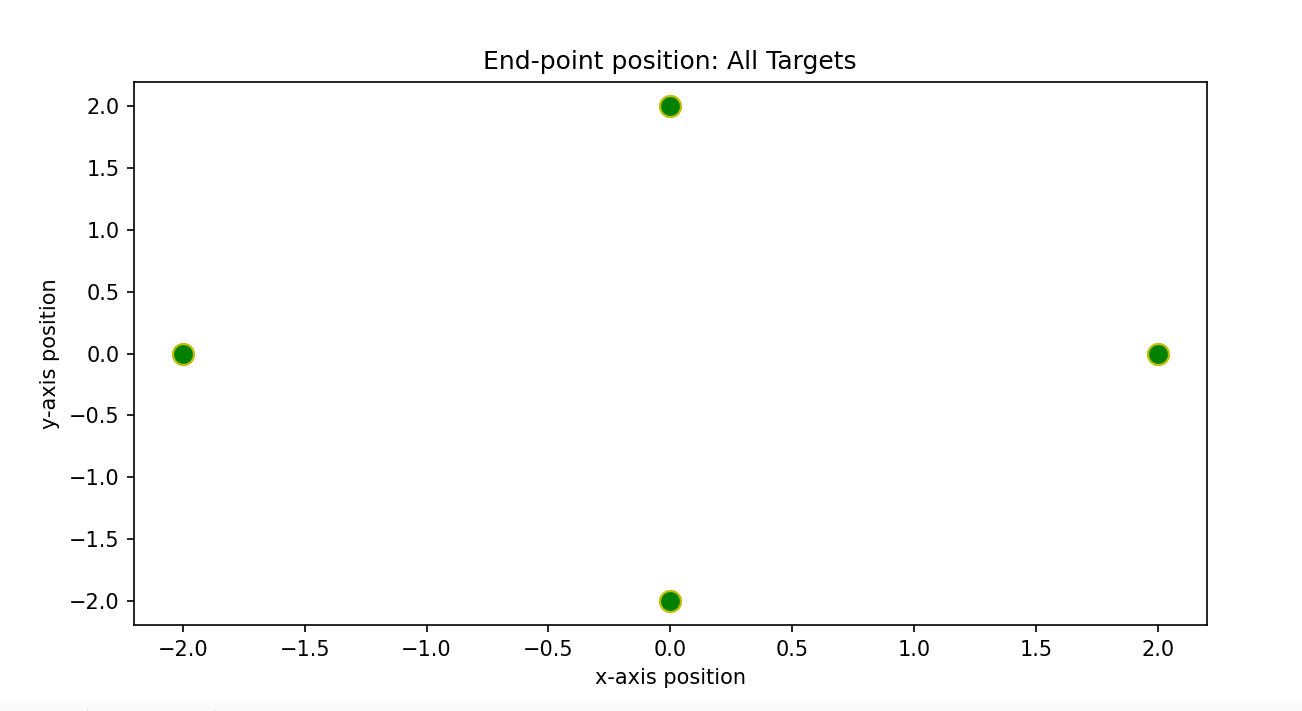
\includegraphics[width=0.5\textwidth]{points-4}}
		\subfloat{
			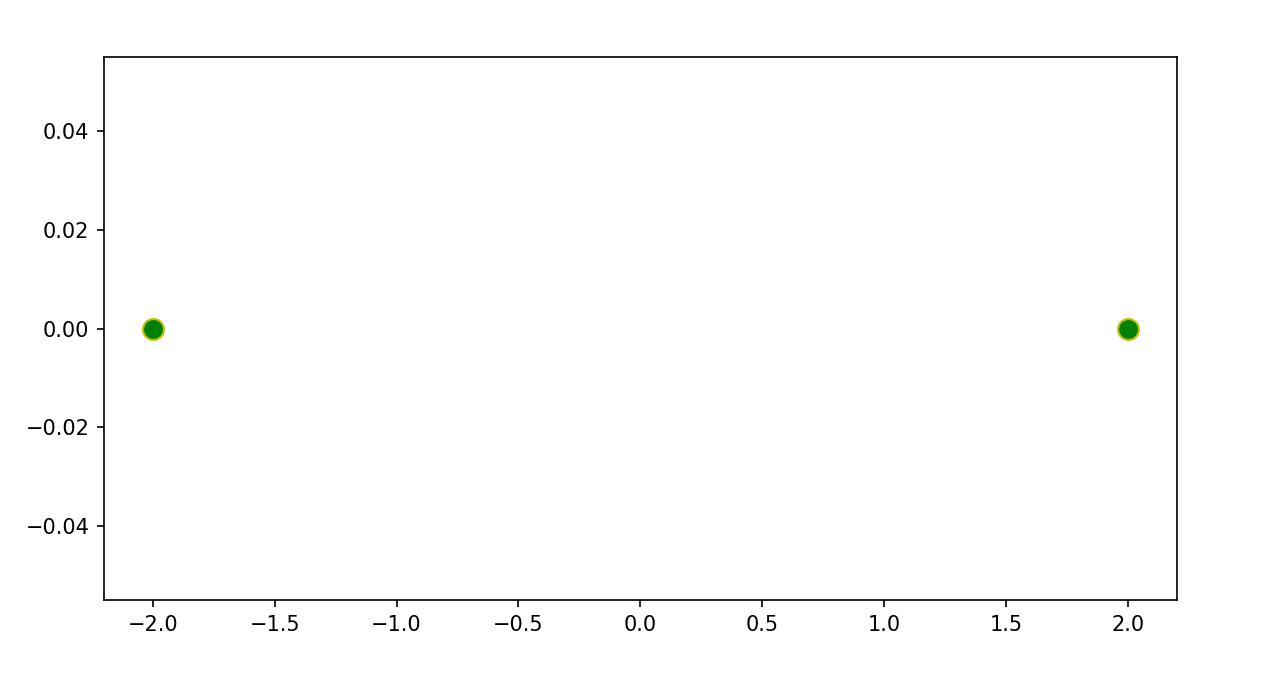
\includegraphics[width=0.5\textwidth]{puntos2}}
	\end{figure}
	
\end{frame}
\begin{frame}
	\frametitle{Desarrollo}
	\begin{itemize}
		\item \textbf{Callbacks}
		\begin{itemize}
			\item Síncronas o asíncronas
			\item Con return code DONE o CONTINUE
			\item Algunos ejemplos:
			\begin{itemize}
				\item beginUpdateCallback (asíncrona, continue)
				\item forceCallback (asíncrona, continue)
				\item actionInitialized (asíncrona, done)
				\item actionFinished (asíncrona, done)
				\item setDeviceTransformationCallback (síncrona, done)
			\end{itemize}
		\end{itemize}
		
	\end{itemize}
	
\end{frame}

\begin{frame}
	\frametitle{Fase 4: con fuerza y sin cursor}
	\begin{columns}
		\begin{column}{0.5\textwidth}
			\begin{figure}[t]
				\includegraphics[width=0.88\textwidth]{sujeto1/force_no_cursor/trayectorias}
				\includegraphics[width=0.88\textwidth]{sujeto2/force_no_cursor/trayectorias}
				\includegraphics[width=0.88\textwidth]{sujeto4/force_no_cursor/trayectorias}
			\end{figure}
		\end{column}
		\begin{column}{0.5\textwidth}
			\begin{figure}
				\includegraphics[width=\textwidth]{sujeto3/force_no_cursor/trayectorias}
				\includegraphics[width=\textwidth]{sujeto5/force_no_cursor/trayectorias}
			\end{figure}
		\end{column}
	\end{columns}
\end{frame}


\begin{frame}
	\frametitle{Fase 3: sin fuerza y sin cursor}
	\begin{columns}
		\begin{column}{0.5\textwidth}
			\begin{figure}[t]
				\includegraphics[width=0.88\textwidth]{sujeto1/no_force_no_cursor/trayectorias}
				\includegraphics[width=0.88\textwidth]{sujeto2/no_force_no_cursor/trayectorias}
				\includegraphics[width=0.88\textwidth]{sujeto4/no_force_no_cursor/trayectorias}
			\end{figure}
		\end{column}
		\begin{column}{0.5\textwidth}
			\begin{figure}
				\includegraphics[width=\textwidth]{sujeto3/no_force_no_cursor/trayectorias}
				\includegraphics[width=\textwidth]{sujeto5/no_force_no_cursor/trayectorias}
			\end{figure}
		\end{column}
	\end{columns}
\end{frame}

\begin{frame}
	\frametitle{Sujeto 1}
	\begin{figure}
		\centering
		
		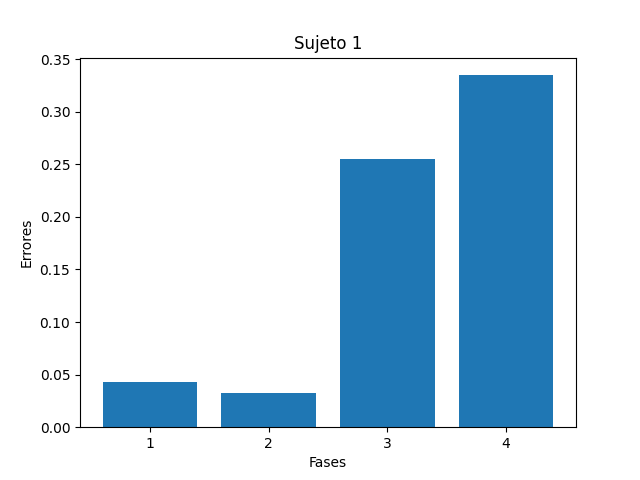
\includegraphics[width=0.45\textwidth]{sujeto1-errores}
		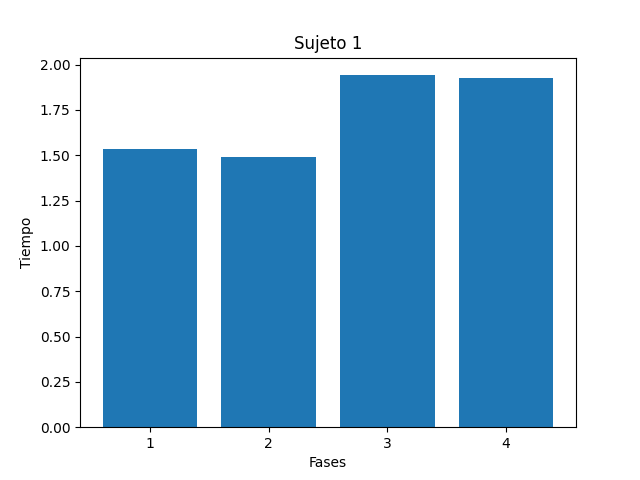
\includegraphics[width=0.45\textwidth]{sujeto1-time}
	\end{figure}
	\begin{itemize}
		\item Cuando se muestra el cursor el aprendizaje se extrapola directamente de la fase 1 a la 2, sin embargo cuando no se muestra el cursor el error crece.
	\end{itemize}
\end{frame}
\begin{frame}
	\frametitle{Sujeto 2}
	\begin{figure}
		\centering
		
		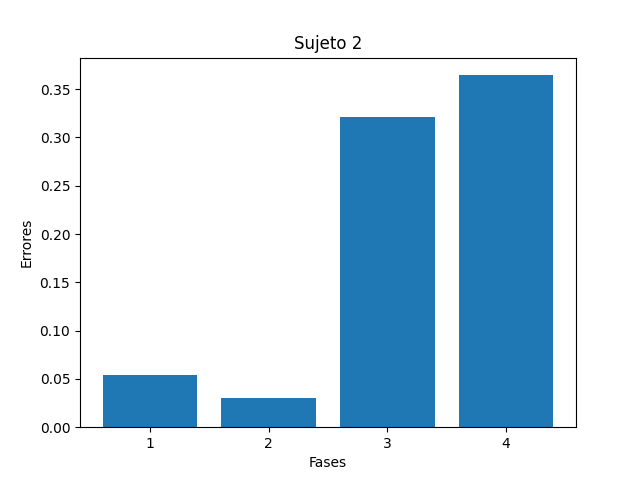
\includegraphics[width=0.45\textwidth]{sujeto2-errores}
		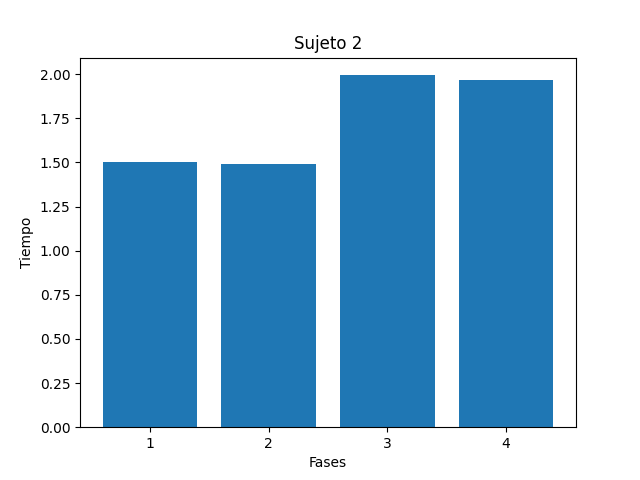
\includegraphics[width=0.45\textwidth]{sujeto2-time}
	\end{figure}
	\begin{itemize}
		\item Resultados muy similares al sujeto 1: no afecta que los targets aparezcan en orden o de forma aleatoria.
	\end{itemize}
\end{frame}
\begin{frame}
	\frametitle{Sujeto 3}
	\begin{figure}
		\centering
		
		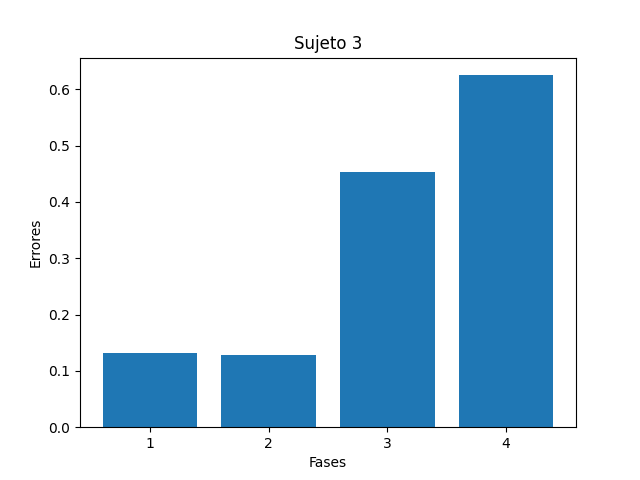
\includegraphics[width=0.45\textwidth]{sujeto3-errores}
		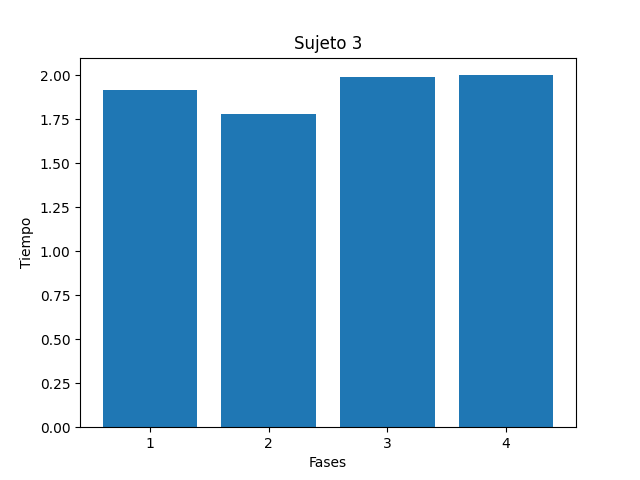
\includegraphics[width=0.45\textwidth]{sujeto3-time}
	\end{figure}
	\begin{itemize}
		\item Los errores crecen, pero el patrón se mantiene: resultados parecidos entre las fases 1 y 2; y sin embargo peores resultados de la fase 4 respecto a la 3.
	\end{itemize}
\end{frame}
\begin{frame}
	\frametitle{Sujeto 4}
	\begin{figure}
		\centering
		
		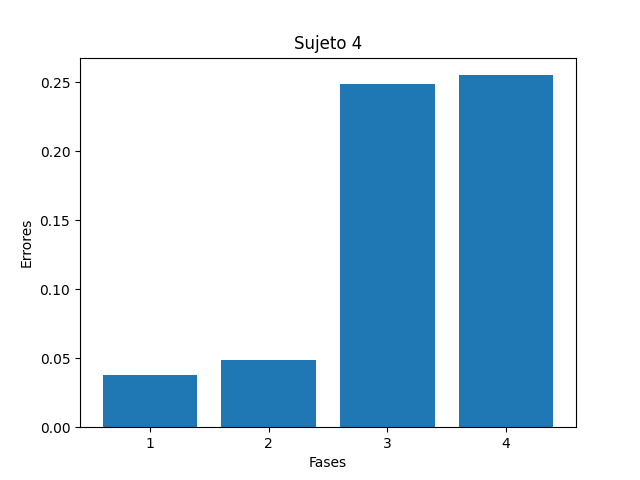
\includegraphics[width=0.45\textwidth]{sujeto4-errores}
		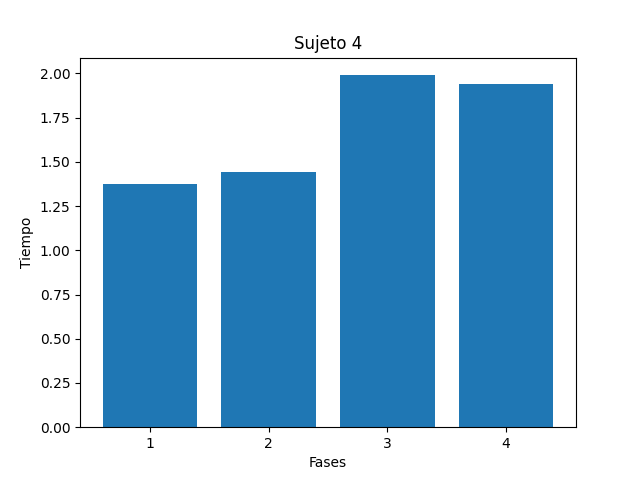
\includegraphics[width=0.45\textwidth]{sujeto4-time}
	\end{figure}
	\begin{itemize}
		\item Sujeto en el que menos se puede apreciar el efecto de la fuerza aplicada: los resultados son prácticamente iguales entre las fases 1 y 2, y las fases 3 y 4.
	\end{itemize}
\end{frame}
\begin{frame}
	\frametitle{Sujeto 5}
	\begin{figure}
		\centering
		
		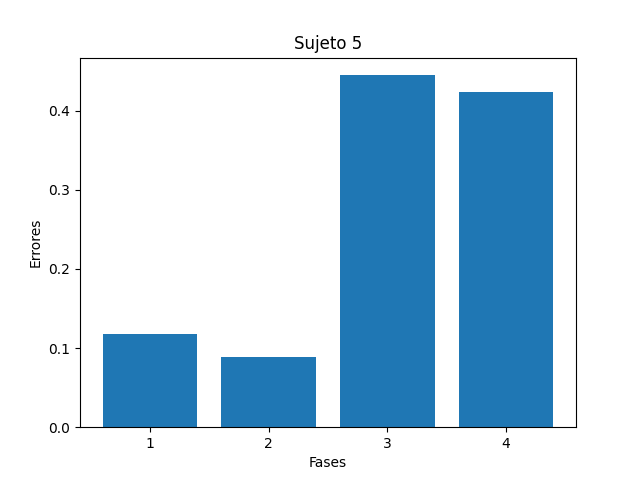
\includegraphics[width=0.45\textwidth]{sujeto5-errores}
		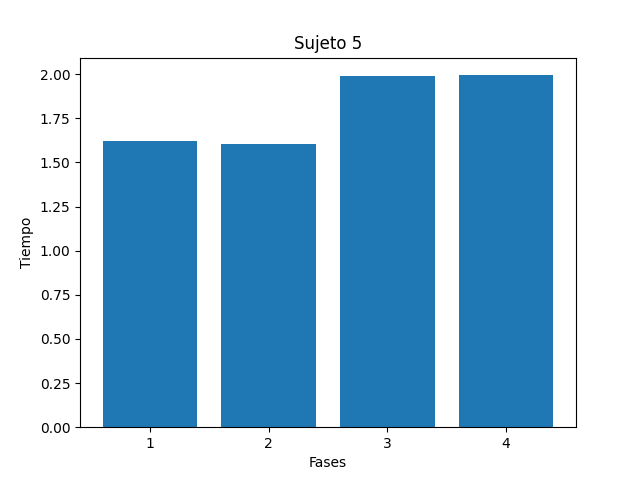
\includegraphics[width=0.45\textwidth]{sujeto5-time}
	\end{figure}
	\begin{itemize}
		\item Único sujeto en el que no crecen los errores de la fase 4 respecto a la fase 3.
	\end{itemize}
\end{frame}